\XtoCBlock{Outport}
\label{block:Outport}
\begin{figure}[H]
\includegraphics{Outport}\end{figure} 

\begin{XtoCtabular}{Outports}
OUT & Signal to frame program\tabularnewline
\hline
\end{XtoCtabular}


\begin{XtoCtabular}{Mask Parameters}
ts\_fact & Multiplication factor of base sampling time (in integer format)\tabularnewline
\hline
Gain & Gain value used in simulation\tabularnewline
\hline
Offset & Offset value used in simulation\tabularnewline
\hline
Delay & Time delay of signal used in simulation\tabularnewline
\hline
\end{XtoCtabular}

\subsubsection*{Description:}
Serves as interface to the frame program. The output of this block is intended for simulation purposes and can be left unconnected if not used. Also the parameters \textit{Gain}, \textit{Offset}, and \textit{Delay} are only used during simulation. The schematic for simulation can be seen in the figure below.
\begin{figure}[H]
  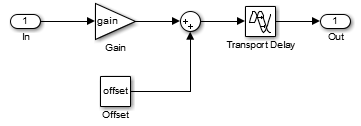
\includegraphics{Outport_Schematic}
\end{figure}

\subsubsection*{Data Types:}
\begin{tabular}{l l}
\textbf{int8} & 8 Bit Fixed Point\tabularnewline
\textbf{int16} & 16 Bit Fixed Point\tabularnewline
\textbf{int32} & 32 Bit Fixed Point\tabularnewline
\textbf{float32} & 32 Bit Floating Point\tabularnewline
\textbf{float64} & 64 Bit Floating Point\tabularnewline
\end{tabular}
